
 In the second calibration all the agents in the economy have the same discount rate. This is chosen to give a much higher transitory consumption elasticity, close to what we see in the data. To generate such a high elasticity it is necessary to introduce an unfeasibly low discount factor. In the following sections we will show how a model of this type could possibly be reconciled with the data.
Table \ref{table:simulation_psi} shows the estimates of $\psi$ using simulated data. The left hand panel shows the calibration to match the distribution of liquid assets. Here we see that using $n1=3$ and $n2=5$ underestimates the true elasticity, giving a value of 0.34 versus the `true' value of 0.38 obtained as $n1$ gets large (and hence the assumption that the consumption response lasts no longer that $n1-1$ years holds true). Thus, if this model was an accurate representation of the economy we would need to use a larger value of $n1$ or risk underestimating $\psi$. In the data we find our estimate for $\psi$ is in fact much \textit{larger} than implied by this model. In the second calibration the simulated estimate using $n1=3$ and $n2=5$, at 0.78, is very close to the `true' value of 0.79.
\begin{center}
	\input\econtexRoot/Tables/experimental/Psi_array2.tex	\input\econtexRoot/Tables/experimental/Psi_array1.tex
	\captionof{table}{Simulation estimates of $\psi$}
	\label{table:simulation_psi}
\end{center}
Table \ref{table:empirical_psi} shows how the estimate of $\psi$ varies when using different values of $n1$ and $n2$ in the data. The estimates around $n1$=3 and $n2$=5 are relatively stable at 0.76, but grow significantly as $n1$ increases beyond 5. This is likely due to the permanent shock in fact having some slow reversion to the mean that makes the method unreliable for larger values of $n1$. Appendix ****** shows that when permanent income follows an AR(1) process with persistence 0.95, the method is accurate for small values of $n1$ but becomes significantly upward biased as $n1$ gets large. This creates a tension between choosing $n1$ low enough to avoid this bias, but high enough such that we allow time for the consumption response to die and do not underestimate the coefficient.
\begin{center}
	\input\econtexRoot/Tables/experimental/Psi_array_empirical.tex		\captionof{table}{Empirical Estimates of $\psi$}
	\label{table:empirical_psi}
\end{center}
Table \ref{table:simulation_phi} shows the results of the simulation for the consumption elasticity to the permanent shock. Here we see very reliable estimates for any choice of $n1$ and $n2$ we care to make. Agents in the model adjust permanent consumption one for one with permanent income (in the medium run) and this comes through clearly in the estimates. The empirical counterpart to this, table \ref{table:empirical_phi}, also shows robustness to the choice of $n1$ and $n2$, apart from for larger values of $n1$. This is likely due to the same reason as the upward bias of $\psi$ for large $n1$, namely that the permanent shock is not entirely permanent.
\begin{center}
	\input\econtexRoot/Tables/experimental/Phi_array2.tex	\input\econtexRoot/Tables/experimental/Phi_array1.tex
	\captionof{table}{Simulation Estimates of $\phi$} 
	\label{table:simulation_phi}
\end{center}

\begin{center}
	\input\econtexRoot/Tables/experimental/Phi_array_empirical.tex		\captionof{table}{Empirical estimates of $\phi$}
	\label{table:empirical_phi}
\end{center}

\subsection{Preference Shock Model with Elastic Labor Supply} \label{pref_shock_model}
The empirical results of this paper suggest that the consumption response to a transitory shock to income lies at the high end of the existing literature. In this section we try to reconcile the results we get with the existing literature by asking if we can build a model in which our empirical method would estimate much larger elasticities than more traditional approaches to measuring the marginal propensity to consume out of transitory shocks. The intuition we build upon is that the households may wish to work longer hours, and hence earn more, in years when their expenditure is particularly high. If this were the case the income process would not be well modeled as being exogenous and our method would have a reverse causality problem embedded in it. Here we build such a model and see how much reverse causality can plausibly contribute to the results we obtain.
The model extends the standard incomplete markets model from section \ref{standard_model}, incorporating both preference shocks, so that households have some years when their utility of consumption is greater than others, and labor elasticity, so that households can adjust their income based on the marginal utility of consumption. The household's problem is to maximize expected lifetime utility:
\begin{align*}
\mathbb{E}_t \sum_{n=t}^{\infty} \beta^n \Bigg(\mathcal{X}_n \frac{ \cLevBF_n^{1-\rho}}{1-\rho}-\frac{\lLevBF_n^{1+\frac{1}{\xi}}}{1+\frac{1}{\xi}} \Bigg)
\end{align*}
subject to the constraints:
\begin{align*}
\aLevBF_t = \mLevBF_t - \cLevBF_t \\
\bLevBF_t = R\aLevBF_t \\
\yLevBF_t =  l_t w_t \\
\lLevBF_t = l_t \pLevBF_t^{\frac{1-\rho}{1+\frac{1}{\xi}}}\\
w_t = \theta_t \pLevBF_t \\
\pLevBF_t = \Psi_t \pLevBF_{t-1} \\
\mLevBF_t = \bLevBF_t + \yLevBF_t
\end{align*}
The normalization of labor $(\lLevBF_t = l_t \pLevBF_t^{\frac{1-\rho}{1+\frac{1}{\xi}}})$ is set up to allow labor supply to move elastically with transitory income, but the long run supply of labor does not depend on permanent income (as observed in the consistency of hours worked over long time periods and across countries). The key additional features of this model are i) the preference shock factor and ii) the elasticity of labor.

The preference shock factor, $\mathcal{X}_t$, multiplies the marginal utility of consumption in that period. When it is high the effective discount factor for consumption between this period and next is low so households will wish to spend much of their resources this period and will have little incentive to save for the next period. Equivalently when it is low, households will prefer to delay consumption to the following periods. There is little empirical evidence on the size of preference shocks, largely because consumption data usually has so much measurement error that estimating the standard deviation of consumption growth is very difficult. While a model with no preference shocks will normally imply a consumption path that is significantly smoother than the income process, our data suggests the standard deviation of income growth is 0.12 while the standard deviation of consumption growth is 0.37. Such a high standard deviation in consumption growth is likely to be mostly driven by measurement error on the asset side of the balance sheet, but it is certainly consistent with very large preference shocks. In our simulations we consider annualized preference shocks with standard deviations up to 0.5.

Labor elasticity is controlled by the Frisch elasticity $\xi$. When the wage (relative to permanent income) increases by $x\%$, hours worked increase by $\xi\%$. Estimates of the Frisch elasticity in micro-data studies range from 0 to 0.5, while macroeconomic studies generally find a much larger elasticity of between 2 and 4 (see \cite{peterman_reconciling_2016}). We will study a range of elasticities between 0 and 1, easily covering the microeconomic estimate range. We will not consider estimates of the Frisch elasticity in the macroeconomic range as it seems likely to us that these estimates are high due to labor market frictions over the business cycle, rather than genuine labor supply choices of households.

\begin{center}
	\input\econtexRoot/Tables/experimental/beta_laborsupply.tex	
	\input\econtexRoot/Tables/experimental/TranShk_laborsupply.tex		\captionof{table}{Fitted discount factors and transitory shock standard deviation}
	\label{table:fitted_beta_and_transtd}
\end{center}

\begin{center}
	\input\econtexRoot/Tables/experimental/phi_laborsupply.tex	
	\input\econtexRoot/Tables/experimental/c_std_laborsupply.tex		\captionof{table}{Simulation estimates of $\phi$ and consumption growth standard deviation}
	\label{table:phi_laborsupply}
\end{center}

\begin{center}
	\input\econtexRoot/Tables/experimental/mpc_laborsupply.tex
	\input\econtexRoot/Tables/experimental/psi_laborsupply.tex		\captionof{table}{Simulation estimates of 6 month MPC and $\psi$}
	\label{table:psi_mpc_laborsupply}
\end{center}

In tables \ref{table:fitted_beta_and_transtd}, \ref{table:phi_laborsupply} and \ref{table:psi_mpc_laborsupply} we have varied the size of the Frisch elasticity and annualized preference shock. In each cell we have kept constant the overall annualized income growth variance and the median liquid asset to annual income ratio (equal to 0.2 in the data). To achieve this we vary the discount factor and the variance of transitory wage shocks.

Table \ref{table:fitted_beta_and_transtd} shows how the discount factor, $\beta$ and the annualized transitory shock standard deviation vary. As the size of the preference shocks increase, so does the precautionary motive for households. As we have fixed the median amount of precautionary savings, the discount factor drops significantly to compensate. This effect is most prominent when there is no labor elasticity. As labor elasticity increases households are able to insure themselves against preference shocks with their labor supply, so the change in discount rate is less pronounced. The right hand panel shows the standard deviation of transitory shocks required to match the overall level of income growth variance goes down as labor supply elasticity increases. This is as expected - when the transitory wage is low households will work fewer hours. This amplifies the variance of the transitory income shock relative to the wage shock. The size of the preference shocks have little effect on the imputed size of the transitory shocks, except when both the preference shock and the labor elasticity are large. At this point the preference shocks themselves induce significant changes in hours worked and hence income, requiring less exogenous variance in income to match the total income variance target.

The left hand panel of table \ref{table:phi_laborsupply} shows the estimate of $\phi$ (the consumption elasticity to permanent shocks) is close to 1 for variations of preference shocks and labor elasticities. This is unsurprising as labor does not respond to a change in permanent income. The right hand panel shows a very significant increase in the standard deviation of consumption growth as the size of the preference shocks increases. With no preference shocks, the standard deviation of consumption growth (0.05) is about half of the standard deviation of income (0.12). As the size of preference shocks increases, so does consumption growth variance, with the standard deviation growing to 0.23 for large preference shocks. This is still much smaller than 0.37, which comes directly from the data, although this high number from the data is likely to be contaminated with measurement error in assets. A further consideration is that much of the observed variance in expenditure growth will be due to durable items, such as home improvements and vehicles. We analyze the effect of durables on our estimates in section \ref{durables}, but to the extent that these goods can be financed, our model with no borrowing may overestimate both the expenditure variance and the labor supply response to preference shocks.

Table \ref{table:psi_mpc_laborsupply} compares the actual mean six month MPC in the model with our empirical method for estimating the transitory expenditure elasticity. While these concepts are clearly not equivalent, comparing the two gives a good understanding as to what might be going on. The left hand panel shows that both preference shocks and labor elasticity, often both missing in consumption models for simplicity, have quantitatively significant impacts on the implied marginal propensity to consume. Increasing the Frisch elasticity from 0 to 0.5 (the full range of micro-estimates) decreases the six month MPC from 17\% to just 8\%. This is because households now have an extra tool with which to insure against low consumption. When they receive a negative transitory shock to their wealth, they will consume less, which in turn will increase their marginal utility of consumption and induce them to work more hours. Therefore their actual income loss will be lower than the shock to their wealth and they will reduce their consumption by less than if they were unable to adjust their labor supply. In contrast, increasing the size of the preference shocks greatly increases the marginal propensity to consume. This is a result of the higher precautionary savings motive and consequently lower discount factor, even while median savings are unchanged. Households with a large positive preference shock will have very little motive to save, as with such low level of savings they will soon get close to the natural borrowing constraint with an MPC close to unity. Many recent papers, such as \cite{krueger_macroeconomics_2016}, have attempted to carefully quantify the macroeconomic dynamic consequences of a serious heterogeneous agent model, but thus far have not included significant preference shocks in their calibrations. The evidence here suggests that such shocks may have a quantitatively important role to play, especially in increasing the marginal propensity to consume. To the extent that the precautionary motive is driven by preference shocks as opposed to income shocks, social insurance for unemployment will not reduce precautionary savings as much as these models presently suggest.

The right hand panel of table \ref{table:psi_mpc_laborsupply} shows the effect of preference shocks and labor elasticity on our empirical estimates of $\psi$, the transitory expenditure elasticity. The top row shows that our estimate is lower than the six month MPC (due to the fact that at these low levels of MPC, more than three years is required for the transitory effect to decay away). It does however follow the same pattern as the MPC and falls in magnitude as the ability of households to adjust labor supply increases. Similarly, going down the first row shows that the estimated expenditure elasticity increases with the preference shock. However, the similarity to the MPC table ends when we increase \textit{both} labor elasticity \textit{and} the size of the preference shocks. Our estimate can grow large, up to a value of 0.64, getting close to our empirical estimates, when the Frisch elasticity is 0.5 and the preference shock standard deviation is 0.4. This measured consumption elasticity to transitory income shocks now bears little relation to the six month MPC (which is 0.16). Instead it is being driven by reverse causality, whereby preference shocks are driving consumption along with the decision to increase labor. The observed `shocks' to income are therefore highly correlated with consumption, but they are not causing the consumption dynamics exogenously.


\subsection{Robustness to Misspecification} \label{misspecification}
In general the estimated permanent and transitory shock variance will be sensitive to the exact assumptions made about the income process. For example allowing the permanent component to mean revert (as in \cite{ahn_when_2017} or \cite{arellano_earnings_2017}) or allowing for correlation between the permanent and transitory shocks will affect how the total observed variance is divided between permanent and transitory. However, as the estimates we obtain for transitory and permanent MPX are close to equal to each other these results are relatively robust to different specifications of the income process.\footnote{We plan to carry out a number of robustness tests by changing the assumptions made about both the income and consumption processes. Our initial results suggest the estimated variances can change significantly, but the estimated MPX numbers are relatively robust.}

A key part of our identification method is the assumption that the impulse response for both income and consumption to a transitory shock has decayed to zero two years after the initial shock. We used growth over 3, 4 and 5 years for our identification because three years is the minimum to allow for generic impulse responses up to two years and demanding that households have more than five years of continuous data reduces the sample and possibly introduces sample selection problems. Figure \ref{fig:IncreasingDiff} makes use of the fact that our model is overidentified with the rich data available to us, so we can test some of this assumption. The solid black line shows the empirically measured variance of income growth over 1 to 7 years. The solid red line draws the straight line equation \ref{variance} with transitory and permanent variance parameters estimated using minimum distance on 3, 4 and 5 years of income growth. The empirical variance of income growth over two and three years is lower than this red line showing equation \ref{variance} is not valid for $n < 3$, consistent with some persistence in the transitory shock extending out to two years. However, the empirical variance over 6 and 7 years of income growth falls almost exactly on the red line implied by the model. This is strong evidence that the transitory component and income does not persist more than two years and that the permanent component does not mean revert at any significant rate.\footnote{We plan to carry out formal overidentification tests here. As we have so much data it is very likely that such a test suggest our model is misspecified. This would not be a concern (all models are simplifications) unless it is economically significant, something figure \ref{fig:IncreasingDiff} shows is not the case.}

The dashed black line and solid green line repeat this experiment with the covariance of income and consumption over increasing years of growth. This time the solid green line is equation \ref{covariance} with parameters identified by 3, 4 and 5 years of growth. As with income, the model says that this covariance should grow linearly for $n \geq 3$. The assumption that the transitory consumption response goes to zero within 2 years is less common than the equivalent assumption on income and is key to our identification. The data again show that for $n < 3$ the covariance is below the green line, but that for growth over 6 and 7 years the model does a good job.
\begin{figure} 
	\begin{centering}
		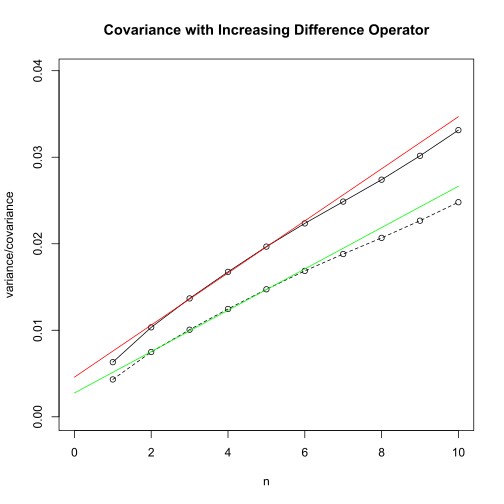
\includegraphics[scale=0.6]{\econtexRoot/Figures/IncreasingDiff_level_lincome_head.png}
		\caption{Variance and Covariance Over n Years of Growth}
		\label{fig:IncreasingDiff}
	\end{centering}
\end{figure}

\subsection{Why is the MPX out of Transitory Shocks so High?} \label{whysohigh}
The results of this paper for permanent shocks is generally in line with both theory and previous empirical work. However, the MPX out of transitory shocks is at the high end of empirical work and is especially high relative to standard consumption theory.

Table \ref{table:MPCLiterature} shows that our estimate of the MPX out of transitory shocks is at the high end, but not extreme. Our measure includes all spending on both durables and non-durables and represents the elasticity of consumption with transitory income received over a full year, a longer period than for many of the estimates in table \ref{table:MPCLiterature}. Estimates from \cite{agarwal_consumption_2014}, \cite{parker_consumer_2013} and \cite{souleles_response_1999} are all similar or higher than ours. However, \cite{fagereng_mpc_2016} estimate much lower MPXs (around 0.4) using well identified lottery winnings in a country (Norway) that is likely more similar to Denmark than the US. Furthermore, the expenditure data they use is imputed in a similar way to ours, so in order to take our results seriously we should have some idea why they may be so different to those from this paper. One answer may be that household's consumption response to a lottery win is different to other types of transitory shocks they may receive. While our initial impression is that households would spend more out of a lottery win (especially if they spend on celebrating the win), it is also possible that households put their winnings into a separate `mental account' (\cite{thaler_mental_1985}) from which they spend less than from their labor earnings. 

Another possibility, that deserves further investigation, is that our method may be picking up reverse causality between income and consumption. In our model, as is common in this literature, we treat the income process as exogenous. However, households may be able to adjust their labor supply in response to shocks. In particular, in years in which households have large spending needs (for example if they buy a car, carry out home improvements or pay for an offspring's wedding) it may be the case that they simultaneously increase their labor supply and hence earnings. Even (or especially) if the labor supply response is small, our model would see that as a very large increase in spending in response to a small increase in income. In future work we plan to address this in a quantitative model in which there are both transitory shocks to income and transitory shocks to consumption preferences. It is unclear to us at the moment how quantitatively important such a mechanism may be. Some empirical evidence that this mechanism may be important is that in households with two earners, the MPX out of transitory shocks from the secondary earner is significantly higher than for the primary earner. It is well established that the labor elasticity of secondary earners is higher than for primary earners so the possibility of reverse causality may be stronger for them.

A final possibility is that measurement error is driving our results to some extent. Our method is robust to classical measurement error in consumption. The permanent MPX is robust to classical measurement error in income while the transitory MPX would be biased downwards with classical measurement error in income uncorrelated with consumption. However, our method of imputing expenditure from income and wealth will pass any measurement error in income over to expenditure. Thus the portion of transitory income variance that is due to measurement error will have a related MPX of 1. Due to the fact that our income data comes from third party reported tax data we believe this portion is likely very small. We plan to investigate this by reducing the sample to households for whom we have reason to believe our income data is particularly accurate. A further test we plan to carry out is to use car purchases instead of total expenditure. Register data on car purchases are available from the Danish car registry. This gives us a source of very well measured expenditure totally independent of our imputed expenditure method. This will act as a robustness test to our surprising result that even households with high levels of liquid wealth have expenditure tied closely with income.

\subsection{Robustness to Auto Regressive Permanent Income}
The previous sections attempted to reconcile the results we obtain with modern consumption savings models. Our conclusion from that exercise is that these models cannot reproduce the observed results unless we assume empirically unrealistic levels of preference shocks and income elasticity. In the models we considered we did not change the income process, which we assumed consisted of both a permanent and a transitory component. In this section we will consider non-structural models, closer to that of our empirical method itself, but instead explore how misspecification in the income process may affect our results. In particular we will simulate a model of the form:
\begin{align*}
p_{t} = \rho p_{t-1} + \varepsilon_{t} \\
y_t = p_t + q_t \\
c_{t} = \phi y_t + \psi q_t
\end{align*}
where $p_t$ is the log of permanent income, $y_t$ the log of total income, and $q_t$ a transitory shock to income. We choose the variance of the permanent and transitory shocks to be equal. We also set the consumption elasticity to permanent shocks, $\phi$ to be 0.8 (to match our empirical results) and the consumption elasticity to transitory shocks, $\psi$, to be 0.4. This is chosen to be closer to the rest of the empirical literature on marginal propensities to consume. We are interested in seeing if our empirical method may significantly bias this 0.4 value in the case that the income process is misspecified.

\begin{center}
	\input\econtexRoot/Tables/experimental/phi_AR1.tex	
	\input\econtexRoot/Tables/experimental/psi_AR1.tex		\captionof{table}{Estimates with AR(1) income process}
	\label{table:AR1}
\end{center}

Table \ref{table:AR1} shows the results of our simulation for various values of $\rho$ and $n_1$ ($n_2$ is always chosen to be $n_1+2$). Remember in our core results we use values of $n_1=3$ and $n_2=5$. The left hand panel of table \ref{table:AR1} shows the misspecification of the income process does not bias the estimate of $\phi$. However, the right hand panel shows a slight upward bias for our estimate of $\psi$ as the value of $\rho$ decreases. This bias increases with the value of $n_1$. This is because the total income variance does not grow linearly with time. Instead the growth in variance starts to taper off as the period of over which income growth is measured increases. This leads to the empirical methodology interpreting much of the `permanent' variance as transitory, and associating a higher consumption elasticity with it. This effect is small for reasonable values of $\rho$ at $n_1=3$. Furthermore as the difference between the true $\phi$ and $\psi$ becomes smaller, so does this bias. When $\phi=\psi$ there is no bias at all, as it makes no difference if the empirical methodology interprets the income variance as permanent or transitory.

\subsection{Durables} \label{durables}
A further critique of our empirical methodology is that it does not take account of durable goods, while our data includes all spending (except on real estate) and therefore includes large and durable goods such as cars and home improvements. The empirical model assumes that in response to a transitive income shock, expenditure increases temporarily for up to two years. This is entirely consistent with a model that includes durable goods. However, the model assumes that in response to a permanent shock to income, expenditure increases once to a new permanent level. A model that included permanent goods would instead imply a large one off expenditure on durable goods to get the household up to their desired stream of durable good services, followed by a decrease back to a permanent level of spending that accounts for replenishing the higher level of depreciating durable goods.

To make this idea more explicit, it will help to write down a simple model. The model will show that our empirical methodology continues to estimate the consumption elasticities to permanent and transitory shocks, but that these need to be interpreted carefully. The model uses the same income process as section \ref{BPP_cont} and takes the same shortcuts, working in logs rather than levels. The same ideas as in appendix \ref{sec:Identification} can be used to formalize this model in levels. Remembering the income process is made up of two martingale processes, $P_t$ and $Q_t$, which may have jumps. Instantaneous income is given by:
\begin{align*}
dy_t = \Big( \int_{0}^{t}dP_s \Big) dt  +dQ_t 
\end{align*}
while instantaneous expenditure now has both a durable and non-durable component:
\begin{align*}
dc_t = \phi_{nd} \Big( \int_{0}^{t} dP_s  \Big) dt + \phi_{d} dP_t + \psi dQ_s
\end{align*}
Here we have assumed that the expenditure response to transitory shocks is instantaneous, but it would not change things to assume as before that the response decays to zero after two years. However, it is important that the durable component of the expenditure response to permanent shocks occurs instantaneously with the shock (or very soon after). Aggregating income and consumption annually gives:
\begin{align*}
\Delta^N \bar{y}_T &=  \Big(\int_{T-N-1}^{T-N} (s-(T-N-1))dP_s  + \int_{T-N}^{T-1}dP_s + \int_{T-1}^{T} (T-s)dP_s \Big) \\
& \qquad + \Big(\int_{T-1}^{T} dQ_t -\int_{T-N-1}^{T-N} dQ_t \Big) \\
\Delta^N \bar{c}_T &= \phi_{nd} \Big(\int_{T-N-1}^{T-N} (s-(T-N-1))dP_s  + \int_{T-N}^{T-1}dP_s + \int_{T-1}^{T} (T-s)dP_s \Big) \\
& \qquad + \phi_d \Big(\int_{T-1}^{T} dP_t -\int_{T-N-1}^{T-N} dP_t \Big) \\
& \qquad + \psi \Big(\int_{T-1}^{T} dQ_t -\int_{T-N-1}^{T-N} dQ_t \Big) \\
\end{align*}
From this we can calculate the covariance:
\begin{align*}
\mathrm{Cov}(\Delta^n \bar{c_T},\Delta^n \bar{y_T} ) &= \phi_{nd} \mathrm{Var}(\Delta^n \bar{y_T}) \\
& \qquad + \phi_d \Bigg( \int_{T-1}^{T} (T-s) \sigma_P^2 dt - \int_{T-N-1}^{T-N}(s-(T-N-1)) \sigma_P^2 dt \Bigg) \\
& \qquad + \psi\Bigg(\int_{T-1}^{T}  \sigma_Q^2 dt + \int_{T-N-1}^{T-N}\sigma_Q^2 dt\Bigg) \\
&= \phi_{nd} (n-\frac{1}{3})\sigma_P^2 + 0 +  2 \psi \sigma_Q^2
\end{align*}
So the durable component of the covariance cancels out and our identification method correctly identifies $\phi_{nd}$ and $\psi$, but is unable to identify $\phi_d$.


\section{Conclusion}
Our novel method of measuring the consumption response to income shocks, along with its application to Danish registry data, shows that households with little liquid wealth have spending that moves almost one for one with income, while even households with relatively high levels of liquid wealth also tie their spending closely to their income. We have shown serious flaws in previous methods that have tried to uncover this relation by imposing structure on the income and consumption processes. Our method and results have also opened up new questions, including whether it is reasonable to assume income follows exogenous shocks when doing this kind of work. In future work we plan to look more closely at how labor responds to preference shocks and what implications that might have for the macroeconomy. Our results suggest that households may use adjustments in their labor supply as much as their wealth to self-insure. In a recession voluntarily adjusting one's labor supply become much harder to do as work is much less freely available. One response to this may be for households to increase their precautionary savings to protect against future income or spending shocks. Such a mechanism would further dampen aggregate demand and aggregate the recession.
